\documentclass[11pt]{article}

% Change "review" to "final" for final version.
\usepackage[preprint]{acl}

% Standard packages
\usepackage{times}
\usepackage{latexsym}
\usepackage[T1]{fontenc}

\usepackage{microtype}
\usepackage{inconsolata}

% Additional packages
\usepackage{graphicx}
\usepackage{booktabs}
\usepackage{multirow}
\usepackage{amsmath}
\usepackage{url}
\usepackage{tikz}
\usetikzlibrary{arrows.meta, positioning, shapes.geometric}

\title{A PhoBERT-based Approach for Vietnamese Complaint Span Extraction with AI-assisted Annotation on UIT-ViOCD}

\author{
\begin{tabular}{c}
\textbf{Vu Ngoc Bao Thang} \quad
\textbf{Do Luong Phuong Sang} \quad
\textbf{Le Viet Tan} \quad
\textbf{Luu Minh Tan} \\
University of Information Technology, VNU-HCM \\
Vietnam National University, Ho Chi Minh City \\
\end{tabular}
}

\begin{document}
\maketitle

\begin{abstract}
Vietnamese online complaint detection is commonly formulated as a review-level classification task, where a model predicts whether a review contains a complaint. The UIT-ViOCD dataset provides an important benchmark for this setting, but its original labels only indicate whether a review is complaint-related and do not identify the specific textual region that expresses the complaint. This limitation reduces the interpretability and practical usefulness of complaint analysis systems, especially when a review contains both neutral, positive, and negative opinions.

In this work, we extend UIT-ViOCD from review-level complaint detection to complaint span extraction. We construct an AI-assisted complaint span annotation pipeline that annotates complaint expressions, validates character offsets, repairs incorrect offsets when possible, resolves overlapping spans, and converts validated spans into BIO labels with three tags: O, B-COMP, and I-COMP. The resulting data is used to train PhoBERT-based named entity recognition models for extracting complaint spans from Vietnamese e-commerce reviews.

Our experiments show that training on a small pilot set is insufficient for reliable span extraction. A PhoBERT NER model trained on the pilot 100 records without class weights obtains Entity-F1 of 0.0000, while using class-weighted CrossEntropyLoss improves Entity-F1 to 0.1370. After expanding annotation to the full AI-assisted complaint span dataset, the weighted PhoBERT NER model achieves Entity-F1 of 0.8455 and Token-F1 of 0.8620. These results should be interpreted as evaluation on the constructed AI-assisted span dataset: the full span labels are AI-assisted annotations, not fully human gold-standard labels.
\end{abstract}

\section{Introduction}

Online customer reviews are a valuable source of feedback for e-commerce platforms. They reflect user experience with product quality, delivery, packaging, application behavior, customer service, and after-sales support. Among these reviews, complaint reviews are especially important because they reveal concrete problems that sellers, platforms, or service providers need to address. Automatically analyzing complaint reviews can therefore support product monitoring, service improvement, and large-scale customer feedback analysis.

Vietnamese e-commerce reviews are difficult to process automatically. They often contain informal expressions, spelling variants, teencode, abbreviations, inconsistent punctuation, emojis, and code-switching. A single review may also contain mixed sentiment, where users praise one aspect of a product while complaining about another. In addition, complaints are not always expressed with explicit negative keywords; users may imply dissatisfaction through indirect or incomplete expressions. These characteristics make Vietnamese complaint analysis more challenging than standard text classification.

Existing Vietnamese online complaint detection work, including UIT-ViOCD, primarily formulates the task as review-level binary classification \citep{viocd2021}. In this setting, each review is labeled as complaint or non-complaint. This formulation is useful for identifying whether a review contains a complaint, but it does not answer a more fine-grained question: which part of the review expresses the complaint? For example, in a review that contains both a positive product comment and a negative delivery comment, a review-level label only indicates that a complaint exists, while a span extraction system can identify the exact phrase describing the delivery issue.

This study focuses on complaint span extraction for Vietnamese e-commerce reviews. Instead of treating UIT-ViOCD only as a classification dataset, we extend its complaint reviews with span-level annotations. A complaint span is defined as the shortest phrase that still preserves the meaning of the user's complaint or dissatisfaction. The span extraction task is then represented as a BIO sequence labeling problem with three labels: O, B-COMP, and I-COMP.

To build span-level supervision, we design an AI-assisted annotation pipeline for UIT-ViOCD complaint reviews. The pipeline uses a guideline-driven annotation prompt to identify complaint spans and then applies several quality-control steps before training. First, a validator checks JSONL format, record identity, text consistency, span offsets, and label validity. Second, an offset repair step corrects wrong start and end positions when the annotated span text is an exact substring of the source review. Third, overlapping spans are resolved before converting the data into BIO labels. This process produces a full AI-assisted complaint span dataset of 2,854 complaint reviews from UIT-ViOCD.

For modeling, we train PhoBERT-based NER models on the constructed BIO dataset \citep{phobert2020}. Since token classification can be biased toward frequent labels, especially in small-data settings, we evaluate class-weighted CrossEntropyLoss to encourage the model to learn complaint labels more effectively. The experiments compare three stages of the pipeline: a pilot 100-record setting without class weights, a pilot 100-record setting with class weights, and the full AI-assisted complaint span dataset with class-weighted loss.

The main contributions of this work are as follows:
\begin{itemize}
    \item We analyze the limitation of review-level complaint detection in UIT-ViOCD and motivate the need for complaint span extraction.
    \item We construct an AI-assisted complaint span annotation pipeline for Vietnamese e-commerce reviews.
    \item We convert complaint spans into BIO labels using validation, offset repair, and overlap resolving to improve annotation consistency.
    \item We train and evaluate PhoBERT NER models with class-weighted loss on both pilot and full AI-assisted complaint span datasets.
\end{itemize}

\section{Related Work}

Vietnamese online complaint detection has been studied as a text classification problem in user-generated content. The UIT-ViOCD dataset introduced a benchmark for Vietnamese online complaint detection, where each review is labeled as complaint or non-complaint \citep{viocd2021}. This formulation is useful for review-level filtering and monitoring, but it only provides a coarse label for the entire review. It does not identify the exact phrase or region that expresses the user's dissatisfaction. As a result, review-level complaint detection cannot directly explain what the user complains about.

Complaint span extraction addresses this limitation by moving from document-level prediction to token-level or span-level prediction. Instead of predicting only whether a complaint exists, a span extraction model identifies the textual segment that contains the complaint. This is important in Vietnamese e-commerce reviews because a review may contain multiple aspects, mixed sentiment, or both positive and negative comments. In such cases, a binary review label is insufficient for fine-grained analysis.

Pre-trained language models have become a standard approach for Vietnamese NLP. PhoBERT is a RoBERTa-style model pre-trained on large-scale Vietnamese corpora and has been widely used for Vietnamese text classification and sequence labeling tasks \citep{phobert2020}. Since complaint span extraction requires contextual understanding of informal and noisy Vietnamese reviews, PhoBERT is a suitable backbone for token-level complaint extraction.

Sequence labeling is commonly used for span extraction tasks such as named entity recognition. In the BIO tagging scheme, each token is labeled as outside a target span, at the beginning of a target span, or inside a target span. We adapt this formulation to complaint span extraction using three labels: O, B-COMP, and I-COMP. This representation allows a model to recover complaint spans from token-level predictions.

Low-resource span annotation is expensive because it requires annotators to decide exact boundaries, not only class labels. AI-assisted annotation can help accelerate this process, but it must be used carefully. Automatically produced annotations may contain invalid offsets, overly long spans, overlapping spans, or non-exact text matches. Therefore, this work treats AI annotation as an assisted data construction process rather than a source of fully human gold-standard labels. Validation, offset repair, overlap resolving, and partial manual review are used to improve consistency before model training.

\section{Dataset}

This work uses only the UIT-ViOCD dataset. The local data files used in this study contain 5,484 Vietnamese online reviews from four domains: app, cosmetic, fashion, and mobile. Each review contains review text, a tokenized version of the review, a binary complaint label, and a domain label. The original task is review-level complaint detection, where each review is labeled as complaint or non-complaint.

For the revised task, we keep the original review-level labels but use them to select candidate reviews for complaint span annotation. Only reviews labeled as complaint are sent to the span annotation pipeline. The resulting candidate set contains 2,854 complaint reviews, including 2,292 training reviews, 283 validation reviews, and 279 test reviews. Table~\ref{tab:dataset-statistics} summarizes the dataset splits and complaint candidates.

\begin{table}[t]
\centering
\small
\begin{tabular}{llrrl}
\toprule
Dataset & Split & Records & Complaint candidates & Notes \\
\midrule
UIT-ViOCD & Train & 4,387 & 2,292 & Original split \\
UIT-ViOCD & Val & 548 & 283 & Original split \\
UIT-ViOCD & Test & 549 & 279 & Original split \\
\midrule
UIT-ViOCD & Total & 5,484 & 2,854 & Complaint reviews annotated \\
\bottomrule
\end{tabular}
\caption{Dataset statistics for UIT-ViOCD and complaint candidates used for span annotation.}
\label{tab:dataset-statistics}
\end{table}

After annotation and quality control, the full AI-assisted complaint span dataset contains 2,854 records. Among them, 2,773 records contain at least one complaint span and 81 records have no explicit complaint span after annotation. The dataset contains 10,195 complaint spans and 109,783 whitespace tokens. Table~\ref{tab:span-dataset-statistics} reports the main statistics of the constructed span dataset.

\begin{table}[t]
\centering
\small
\begin{tabular}{lr}
\toprule
Metric & Value \\
\midrule
Total records & 2,854 \\
Records with spans & 2,773 \\
Records without spans & 81 \\
Total spans & 10,195 \\
Average spans per record & 3.5722 \\
Total tokens & 109,783 \\
COMP tokens & 82,497 \\
COMP token ratio & 75.15\% \\
\bottomrule
\end{tabular}
\caption{Statistics of the full AI-assisted complaint span dataset.}
\label{tab:span-dataset-statistics}
\end{table}

\subsection{Data Annotation and Label Construction}

A complaint span is defined as the shortest phrase that still preserves the meaning of a user's complaint or dissatisfaction. The goal is not to select the entire review, but to identify the core issue phrase. For example, if a review contains both a product description and a delivery complaint, only the delivery complaint phrase should be annotated as a complaint span.

We construct complaint spans using an AI-assisted annotation pipeline. The annotation guideline instructs the AI tool to select phrases that directly express problems or complaints, avoid selecting praise or neutral descriptions, avoid using standalone emojis as complaint spans, and prefer concise issue-focused phrases. The guideline also requires each span to be an exact substring of the original text. Character offsets follow Python slicing semantics, meaning that the annotated text must satisfy \texttt{text[start:end] == span\_text}.

The raw AI output is validated before it is used for training. The validator checks that each annotation record has the required fields, that the record identifier exists in the source candidates, that the annotation text matches the source text, that spans are lists with valid start and end offsets, that each span text matches the corresponding substring, and that the only span label is COMP. It also checks duplicate and missing records for each annotation batch.

When a span text is correct but its offsets are wrong, an offset repair step attempts to recover the correct start and end positions by exact substring search in the source review. If the span text appears once, the offset is repaired automatically. If it appears multiple times, the closest position to the old offset is selected and recorded in a repair report. If the span text is not an exact substring of the review, the error is left unresolved for manual inspection instead of being guessed.

Some AI-generated annotations contain overlapping complaint spans. Before BIO conversion, overlapping spans are resolved by merging overlapping COMP spans into a single span that covers the union of their character offsets. This step prevents one token from receiving conflicting labels during BIO conversion. After validation, repair, and overlap resolving, all accepted spans are converted into BIO labels. Tokens outside complaint spans are labeled O, the first token overlapping a complaint span is labeled B-COMP, and subsequent tokens in the same span are labeled I-COMP.

The resulting labels are AI-assisted annotations, not fully human gold-standard labels. Automatic validation, offset repair, overlap resolving, and partial manual review are used to improve consistency, but the dataset should be interpreted as a constructed AI-assisted span dataset.

\section{Methodology}

\subsection{Problem Formulation}

Given a Vietnamese e-commerce review \(x = \{w_1, w_2, \ldots, w_n\}\), the goal is to predict a BIO tag sequence \(y = \{t_1, t_2, \ldots, t_n\}\), where each token-level tag \(t_i\) belongs to \(\{O, B\text{-}COMP, I\text{-}COMP\}\). The O label indicates that a token is outside a complaint span, B-COMP indicates the first token of a complaint span, and I-COMP indicates a subsequent token inside the same complaint span.

The main modeling task in this work is complaint span extraction rather than review-level classification. The original review-level complaint labels in UIT-ViOCD are used to select complaint reviews as candidates for span annotation. After candidate selection, the model is trained to identify which tokens in a complaint review express the actual complaint content.

\subsection{AI-assisted Annotation Pipeline}

The proposed data construction pipeline starts from the complaint reviews in UIT-ViOCD. First, reviews labeled as complaints are selected from the original train, validation, and test splits. Second, complaint span annotations are generated with AI assistance using a guideline that defines complaint spans and requires each span to be an exact substring of the source review.

The raw AI annotation output is then processed by a quality-control pipeline. A validator checks the JSONL schema, record identifiers, text consistency, span labels, and exact character offsets. When a span text is correct but the offset is wrong, an offset repair step searches for the exact span text in the original review and updates the start and end positions when this can be done safely. After that, overlapping spans are resolved so that each token receives at most one BIO label. Finally, validated character-level spans are converted into token-level BIO labels and exported as NER JSON files for training and evaluation.

\subsection{BIO Label Construction}

The BIO label set contains three labels. The O label is assigned to tokens outside complaint spans. The B-COMP label is assigned to the first token of each complaint span. The I-COMP label is assigned to the remaining tokens inside the same complaint span. If a review contains multiple complaint spans, each span starts with its own B-COMP tag.

The conversion process uses validated character offsets as the source of truth. Each complaint span is represented as a character interval \([start, end)\). Tokens are generated using whitespace tokenization while preserving character offsets. A token that overlaps the first position of a complaint span receives B-COMP, while later overlapping tokens receive I-COMP. Tokens that do not overlap any complaint span receive O.

Complaint span boundaries are inherently ambiguous in informal Vietnamese reviews. Some reviews contain long explanations, repeated complaints, or mixed positive and negative opinions. For this reason, the annotation guideline prefers concise spans that capture the core issue, while the validation pipeline enforces technical consistency of offsets and labels.

\subsection{PhoBERT NER Model}

The span extraction model uses \texttt{vinai/phobert-base-v2} as the backbone. Each review is first converted into subword tokens by the PhoBERT tokenizer. The tokenized sequence is passed through PhoBERT to obtain contextual token representations. A linear token labeling layer then predicts logits for the three BIO labels: O, B-COMP, and I-COMP.

\begin{figure}[t]
\centering
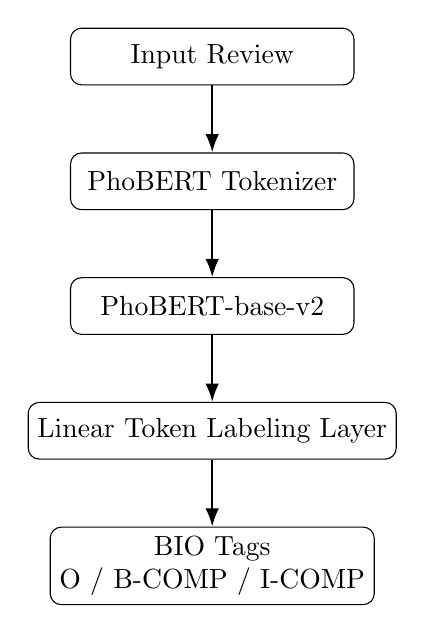
\begin{tikzpicture}[
    node distance=0.85cm,
    box/.style={rectangle, draw, rounded corners, align=center, minimum width=3.6cm, minimum height=0.72cm},
    arrow/.style={-Latex, thick}
]
\node[box] (input) {Input Review};
\node[box, below=of input] (tok) {PhoBERT Tokenizer};
\node[box, below=of tok] (enc) {PhoBERT-base-v2};
\node[box, below=of enc] (head) {Linear Token Labeling Layer};
\node[box, below=of head] (out) {BIO Tags\\O / B-COMP / I-COMP};

\draw[arrow] (input) -- (tok);
\draw[arrow] (tok) -- (enc);
\draw[arrow] (enc) -- (head);
\draw[arrow] (head) -- (out);
\end{tikzpicture}
\caption{PhoBERT NER architecture for complaint span extraction.}
\label{fig:phobert-ner-architecture}
\end{figure}

Since PhoBERT uses subword tokenization, BIO labels must be aligned with subword positions. The first subword of each original token keeps the original BIO label. The remaining subwords and special tokens are assigned the ignore index \(-100\), so they are excluded from loss computation and evaluation decoding.

\subsection{Class-weighted Training Objective}

The model is trained with token-level CrossEntropyLoss. For a token position \(i\), let \(m_i\) be a mask that equals 1 for valid labeled positions and 0 for ignored positions. Ignored positions correspond to labels with value \(-100\). With class weights, the training loss is:

\begin{equation}
L = - \sum_i m_i \, w_{y_i} \log p(y_i \mid x)
\end{equation}

where \(w_{y_i}\) is the weight of the gold BIO label at position \(i\). Class weights are computed from the training split using a balanced scheme:

\begin{equation}
w_c = \frac{N}{K \cdot n_c}
\end{equation}

where \(N\) is the total number of labeled tokens in the training split, \(K\) is the number of classes, and \(n_c\) is the number of training tokens with class \(c\). This weighting scheme reduces the tendency of the model to over-predict frequent labels and encourages learning complaint-related labels.

\subsection{Implementation Details}

The model is implemented using PyTorch and Hugging Face Transformers. All experiments use \texttt{vinai/phobert-base-v2} as the encoder backbone. The batch size is 8 and the learning rate is \(2 \times 10^{-5}\). The pilot 100 setting without class weights is trained for 3 epochs, the pilot 100 weighted setting is trained for 10 epochs, and the full weighted setting is trained for 5 epochs. Experiments are conducted on a Kaggle GPU environment.

The evaluation reports Entity Precision, Entity Recall, Entity-F1, and Token-F1 macro. Entity-level metrics evaluate exact complaint span extraction, while token-level metrics evaluate BIO tagging quality. In the final full-data run, checkpoint saving is disabled to reduce storage usage; metrics and prediction files are still saved for analysis.

\section{Experiments}

We evaluate complaint span extraction as a PhoBERT-based NER task on the AI-assisted BIO datasets constructed from UIT-ViOCD. The experiments are designed to answer three questions. First, whether a small pilot annotation set is sufficient for training a span extraction model. Second, whether class-weighted loss helps reduce label bias. Third, whether expanding annotation to all complaint reviews improves span extraction performance.

\subsection{Experimental Setup}

All experiments use \texttt{vinai/phobert-base-v2} as the backbone and a linear token labeling layer for BIO prediction. The label scheme contains O, B-COMP, and I-COMP. We compare standard CrossEntropyLoss with class-weighted CrossEntropyLoss. For the full weighted experiment, class weights are computed from the training split using the balanced scheme described in Section~4.5. The resulting class counts and weights are: O count = 21,780 with weight 1.342608, B-COMP count = 8,085 with weight 3.616821, and I-COMP count = 57,861 with weight 0.505384.

The batch size is 8 and the learning rate is \(2 \times 10^{-5}\). Experiments are conducted on a Kaggle GPU environment. In the final full-data run, checkpoint saving is disabled to reduce storage usage, while metrics and prediction outputs are still saved for analysis. Table~\ref{tab:experimental-setup} summarizes the experimental setup.

\begin{table}[t]
\centering
\small
\begin{tabular}{ll}
\toprule
Setting & Value \\
\midrule
Backbone & PhoBERT-base-v2 \\
Task & Complaint span extraction \\
Label scheme & O, B-COMP, I-COMP \\
Batch size & 8 \\
Learning rate & \(2 \times 10^{-5}\) \\
Pilot100 unweighted epochs & 3 \\
Pilot100 weighted best epoch & 7 \\
Full weighted epochs & 5 \\
Environment & Kaggle GPU \\
Main metric & Entity-F1 \\
\bottomrule
\end{tabular}
\caption{Experimental setup for PhoBERT NER complaint span extraction.}
\label{tab:experimental-setup}
\end{table}

\subsection{Dataset Splits}

We evaluate two data settings. The first setting uses the pilot 100 AI-assisted annotations, which were created to validate the annotation and BIO conversion workflow. The second setting uses the full AI-assisted complaint span dataset constructed from all 2,854 UIT-ViOCD complaint reviews.

For the full dataset, the NER split contains 2,280 training records, 283 validation records, and 291 test records. The training split contains 87,726 tokens and 65,946 COMP tokens. The validation split contains 10,569 tokens and 8,015 COMP tokens. The test split contains 11,488 tokens and 8,536 COMP tokens. There are no overlapping record identifiers across the train, validation, and test splits.

\subsection{Evaluation Metrics}

We report Entity Precision, Entity Recall, Entity-F1, Token-F1 macro, and average loss. Entity-level metrics require exact span matching and therefore evaluate whether the model extracts the correct complaint span boundaries. Token-F1 macro evaluates BIO tagging quality at the token level and is less strict than exact-span matching. Since complaint span extraction is the main task, Entity-F1 is treated as the primary metric.

\section{Result Analysis and Error Analysis}

\subsection{Overall NER Results}

Table~\ref{tab:ner-results-new} shows the main NER results. The pilot 100 unweighted model fails to extract complete complaint spans, obtaining Entity-F1 of 0.0000 and Token-F1 macro of 0.3002. Adding class-weighted loss improves the pilot setting to Entity-F1 of 0.1370 and Token-F1 macro of 0.5845, but the dataset remains too small for reliable span extraction. The best result is obtained by training on the full AI-assisted complaint span dataset with class-weighted loss, reaching Entity-F1 of 0.8455 and Token-F1 macro of 0.8620.

\begin{table*}[t]
\centering
\small
\setlength{\tabcolsep}{4pt}
\begin{tabular}{lllrrrrr}
\toprule
Experiment & Dataset & Loss & Epoch & Entity-P & Entity-R & Entity-F1 & Token-F1 / Loss \\
\midrule
Pilot100 Unweighted PhoBERT NER & Pilot100 & CE & 3 & -- & -- & 0.0000 & 0.3002 / 0.6437 \\
Pilot100 Weighted PhoBERT NER & Pilot100 & Weighted CE & 7 & 0.0893 & 0.2941 & 0.1370 & 0.5845 / 0.3660 \\
Full Complaint Weighted PhoBERT NER & Full AI-assisted & Weighted CE & 5 & 0.7937 & 0.9045 & 0.8455 & 0.8620 / 0.2486 \\
\bottomrule
\end{tabular}
\caption{NER results for complaint span extraction. The last column reports Token-F1 macro and average loss.}
\label{tab:ner-results-new}
\end{table*}

\subsection{Effect of Class-weighted Loss}

The pilot 100 unweighted experiment shows a strong bias toward the O label. Although the model is trained on annotated complaint reviews, the small number of training examples is not enough for the model to learn reliable B-COMP and I-COMP boundaries. As a result, exact complaint spans are not recovered, leading to Entity-F1 of 0.0000.

Class-weighted CrossEntropyLoss improves this behavior. In the pilot 100 weighted experiment, Entity-F1 increases from 0.0000 to 0.1370 and Token-F1 macro increases from 0.3002 to 0.5845. This suggests that class weighting helps the model start predicting complaint-related labels. However, the result remains limited because the pilot set is small and does not cover enough variation in complaint expressions.

\subsection{Effect of Expanding AI-assisted Span Data}

Expanding annotation from the pilot set to the full AI-assisted complaint span dataset substantially improves performance. The full weighted model reaches Entity Precision of 0.7937, Entity Recall of 0.9045, Entity-F1 of 0.8455, and Token-F1 macro of 0.8620. This improvement indicates that data coverage is critical for complaint span extraction. The full dataset contains more domains, more complaint patterns, and more boundary examples than the pilot set.

The result should be interpreted carefully. The full test set is evaluated against the constructed AI-assisted labels, not against a fully human gold-standard benchmark. Therefore, Entity-F1 of 0.8455 demonstrates strong consistency with the constructed annotation pipeline, but it should not be presented as an official benchmark result for the original UIT-ViOCD dataset.

\subsection{Prediction Distribution Analysis}

Table~\ref{tab:test-label-distribution} compares the gold and predicted label distributions on the full test split at the best epoch. The full test gold labels contain 2,931 O tokens, 1,089 B-COMP tokens, and 7,447 I-COMP tokens. The model predicts 2,392 O tokens, 1,205 B-COMP tokens, and 7,870 I-COMP tokens. It predicts at least one COMP label for 287 out of 291 test samples, while the gold labels contain at least one COMP label for 280 out of 291 samples.

\begin{table}[t]
\centering
\small
\begin{tabular}{lrr}
\toprule
Label & Gold count & Predicted count \\
\midrule
O & 2,931 & 2,392 \\
B-COMP & 1,089 & 1,205 \\
I-COMP & 7,447 & 7,870 \\
\bottomrule
\end{tabular}
\caption{Gold and predicted label distributions on the full test split.}
\label{tab:test-label-distribution}
\end{table}

The predicted distribution shows that the model predicts more complaint tokens than the gold labels. This is partly related to the high COMP token ratio in the constructed dataset, where complaint reviews often contain long or multiple complaint spans. While this behavior improves recall, it can also lead to overly broad span predictions. Therefore, exact boundary evaluation remains important even when token-level scores are high.

\subsection{Error Analysis and Qualitative Discussion}

The main difficulty in complaint span extraction is boundary detection. A model may identify the correct complaint region but include too many surrounding tokens or miss part of the complaint phrase. This affects Entity-F1 more strongly than Token-F1 because entity-level evaluation requires exact span boundaries.

Several error sources remain. First, Vietnamese e-commerce reviews are noisy and informal, with spelling variants, abbreviations, repeated words, and inconsistent punctuation. Second, some reviews contain multiple complaints in a single sentence, making boundary separation difficult. Third, some complaint expressions are implicit or mixed with suggestions, which can make it unclear whether a phrase should be annotated as a complaint span. Finally, because the span labels are AI-assisted, some annotation boundaries may reflect the guideline and validation pipeline rather than fully human consensus.

Overall, the experiments show that class weighting and data expansion are both important. Class weighting helps the model avoid predicting only the dominant label, while the full AI-assisted dataset provides enough span-level supervision for PhoBERT NER to learn complaint extraction patterns.

\section{Conclusion and Future Work}

This work revises Vietnamese complaint analysis on UIT-ViOCD from review-level complaint detection to complaint span extraction. The original UIT-ViOCD labels indicate whether a review contains a complaint, but they do not identify the specific phrase that expresses the complaint. This limitation reduces interpretability and makes the output less actionable for downstream analysis.

To address this issue, we extend UIT-ViOCD with AI-assisted complaint span annotations. The constructed pipeline includes annotation guideline design, schema and offset validation, offset repair, overlap resolving, and BIO conversion. The final AI-assisted complaint span dataset contains 2,854 complaint reviews, including 2,773 records with at least one span, 81 records without explicit spans, 10,195 total spans, and 109,783 tokens. The COMP token ratio is 75.15\%.

We train PhoBERT NER models with token-level BIO labels and class-weighted CrossEntropyLoss. The pilot 100 unweighted model is strongly biased toward the O label and obtains Entity-F1 of 0.0000 and Token-F1 of 0.3002. Using class-weighted loss improves the pilot setting to Entity-F1 of 0.1370 and Token-F1 of 0.5845, but the pilot data remains too small for reliable extraction. Training on the full AI-assisted dataset further improves performance to Entity-F1 of 0.8455 and Token-F1 of 0.8620.

These results show that both class weighting and expanded span-level supervision are important for Vietnamese complaint span extraction. However, the reported scores should be interpreted as evaluation on the constructed AI-assisted span dataset, not as an official benchmark result for the original UIT-ViOCD dataset.

In future work, the full span labels should be reviewed more extensively by human annotators. The annotation guideline can also be refined and evaluated through inter-annotator agreement to improve boundary consistency. Additional quality-control rules may be added to detect broad spans, implicit complaints, and ambiguous span boundaries more strictly. On the modeling side, future experiments can compare the current PhoBERT token classifier with stronger sequence labeling baselines such as PhoBERT+CRF or transformer-CRF models. Another direction is to jointly model review-level complaint classification and span extraction as a future multi-task extension. Finally, error analysis by domain, including app, cosmetic, fashion, and mobile reviews, can help identify domain-specific weaknesses and reduce over-prediction of COMP tokens.

\section*{Limitations}

The main limitation of this work is the nature of the span labels. The full complaint span dataset is built with AI-assisted annotations and is not a fully human gold-standard dataset. Automatic validation ensures that annotation files have valid format, valid offsets, matching span text, and non-overlapping spans, but it cannot guarantee that every span is semantically optimal.

Partial manual review was performed during the pilot and batch expansion process, but not all 2,854 records were fully verified by human annotators. Therefore, some spans may still be too broad, too narrow, or semantically debatable. The high COMP token ratio of 75.15\% also suggests that some annotations may cover relatively large portions of complaint reviews.

The experimental results should be interpreted as performance on the constructed AI-assisted span dataset. In particular, the Entity-F1 score of 0.8455 should not be presented as official benchmark performance on the original UIT-ViOCD task, because the original dataset does not provide human gold-standard complaint span labels.

The model may still struggle with implicit complaints, ambiguous span boundaries, mixed sentiment, informal Vietnamese, spelling errors, teencode, and inconsistent punctuation. In addition, this work focuses on complaint reviews for span extraction; non-complaint reviews are not used for NER training because they do not contain complaint spans in the constructed task.

% Custom bibliography entries only
\bibliography{custom}

\end{document}
